\documentclass[conference]{IEEEtran}
% IEEE format with two-column layout

\usepackage[utf8]{inputenc}
\usepackage{amsmath,amssymb,amsthm,amsfonts}
\usepackage{graphicx}
\usepackage{subcaption}
\usepackage{url}
\usepackage{tikz}

\usepackage{booktabs}
\usepackage{url}
\usepackage{hyperref}
\usepackage{caption}

\usepackage{cite}

\usepackage{ulem}

\usepackage{algorithm}
\usepackage{algpseudocode}

\usepackage{mathtools}
\usepackage{etoolbox}

\makeatletter
\let\lunderbrace\underbrace
\let\runderbrace\underbrace
\let\lupbracefill\upbracefill
\let\rupbracefill\upbracefill
\patchcmd{\lunderbrace}{\upbracefill}{\lupbracefill}{}{}
\patchcmd{\runderbrace}{\upbracefill}{\rupbracefill}{}{}
\patchcmd{\lupbracefill}{\braceru}{\leaders\vrule\@height\ht\z@\@depth\z@\hskip\wd\z@}{}{}
\patchcmd{\rupbracefill}{\bracelu}{\leaders\vrule\@height\ht\z@\@depth\z@\hskip\wd\z@}{}{}
\makeatother

\usepackage{tikz}

\usepackage[a4paper,margin=1in]{geometry}

\usetikzlibrary{matrix,fit,positioning}

\title{\fontsize{18}{22}\selectfont Cool, Chill, and Cruel: Probabilistic Ranking with Greedy \\ Approach for Recovering Sparse Binary Secrets in LWE}
\author{\IEEEauthorblockN{MAMANCHUK Mykola, SID.202420671 \\ Supervising Professor: KUNIHIRO Noboru }
\IEEEauthorblockA{University of Tsukuba / CRISEC}
}
\date{\today}


\usetikzlibrary{matrix,fit,positioning}

% For good measure, define a geometry or margins if you prefer

\begin{document}
\maketitle

\begin{abstract}
  Sparse binary LWE secrets are gaining interest in homomorphic encryption (HE) and post-quantum cryptography due to their efficiency advantages. However, recently proposed attacks (e.g., SALSA, PICANTE, VERDE) have shown that machine learning and statistical methods can compromise such sparse secrets at moderate dimensions. Meanwhile, classical lattice-based cryptanalytic strategies highlight that after partial lattice reduction, certain columns in the LWE matrix remain high-variance (“cruel”), while others become low-variance (“cool”). 
  
  In this work, we refine this approach by introducing a three-region partition—Cruel, Chill, and Cool—aimed at more finely handling columns whose variance slopes rather than sharply dropping. By combining brute force for the cruel region with a probabilistic or ML-based enumeration in the chill region, and a fast greedy bit-flip approach for the cool region, we achieve a flexible attack strategy. 
  
  We provide complexity estimates, schematic diagrams of the multi-zone partition, and discuss potential synergy with ring-based (RLWE) parameter choices, demonstrating how partially reduced columns can be exploited more effectively than prior two-region methods.
  \end{abstract}
  
  \section{Introduction}

  \subsection{Problem Statement and Existing Attacks}
  
  Traditional cryptanalytic efforts on small-secret or sparse LWE include:
  
  \begin{itemize}
      \item \textbf{Primal and Dual attacks}, which reduce the dimension or attempt short-vector recovery \cite{primal-dual}.
      \item \textbf{Hybrid meet-in-the-middle (MiTM) strategies}, which partially guess secret bits and apply lattice reduction on the remainder \cite{hybrid-mitm}.
      \item \textbf{ML-based attacks} (e.g., SALSA, PICANTE, VERDE), which leverage neural networks or transformer architectures to identify correct bits with fewer enumerations \cite{salsa, picante, salsa-verde}.
  \end{itemize}
  
  While these attacks are highly effective, they often treat columns of the partially reduced matrix as simply either “hard” (high variance) or “easy” (low variance). In practice, partial lattice reduction can yield a set of columns whose variances \emph{gradually} decrease, forming a \textbf{sloping} region that does not fit neatly into the typical two-zone (hard vs.\ easy) framework.
  
  \subsection{Our Contribution}
  
  We propose a refined three-zone approach—\textbf{Cruel, Chill, and Cool}—for key recovery in sparse LWE:
  
  \begin{itemize}
      \item \textbf{Cruel region}: columns with variance approximately $\frac{q}{12}$, requiring brute force or meet-in-the-middle strategies.
      \item \textbf{Chill region}: columns exhibiting a moderate variance “slope.” We handle these with a \emph{probabilistic or ML-based} enumeration method, thereby avoiding excessive brute force.
      \item \textbf{Cool region}: columns with significantly reduced variance, recoverable via a simple greedy bit-flip approach.
  \end{itemize}
  
  By partitioning columns more finely, we can reduce the search space in each zone. We provide complexity estimates, illustrate diagrams for this three-zone partition, and discuss how RLWE settings (especially 2-power cyclotomic rings) might be even more susceptible to such a nuanced partial-lattice attack. 
  
  Our method aims to unify insights from recent ML-based approaches with classical partial reduction strategies to more efficiently recover sparse secrets.
  
  \section{Related Work}
  
  \subsection{Existing Lattice-Based Attacks}
  Several known attacks on small or sparse secrets include:
  \begin{itemize}
      \item Primal, Dual, and Hybrid attacks \cite{primal-dual, hybrid-mitm}.
      \item SALSA, a statistical attack leveraging machine learning \cite{salsa}.
      \item PICANTE, which incorporates transformer-based heuristics for LWE key recovery \cite{picante}.
      \item SALSA VERDE, an improved version of SALSA, refining its statistical recovery approach \cite{salsa-verde}.
  \end{itemize}
  
  \subsection{Inspiration for Our Work}
  This work was inspired by the recent research presented in \cite{cool-and-cruel}, which explored the effects of partial lattice reduction on LWE secrets and motivated the three-zone partitioning approach.
  
  \subsection{Conclusion}
  
  We introduce a novel three-zone attack strategy that extends existing binary LWE key recovery methods by partitioning reduced columns into **Cruel, Chill, and Cool** regions. This allows for an adaptive attack leveraging brute-force, probabilistic heuristics, and efficient greedy methods. Our analysis suggests that this approach can improve over traditional two-region models by better handling variance gradients in partially reduced lattices. Future work includes exploring its applicability to structured LWE variants such as Ring-LWE.
  
\section{Preliminaries and Background}
\label{sec:preliminaries}

\subsection{Learning With Errors (LWE)}
\label{subsec:lwe-def}

% Basic definition
LWE in matrix form can be stated as follows. 
Given parameters $(n,m,q)$ and distributions $D_s,D_e$, one samples:
\begin{itemize}
    \item A uniform matrix $\mathbf{A} \in \mathbb{Z}_q^{m \times n}$,
    \item A secret $\mathbf{s} \in D_s \subseteq \mathbb{Z}_q^n$,
    \item A noise (error) vector $\mathbf{e} \in D_e \subseteq \mathbb{Z}_q^m$ (``small'' or low-norm).
\end{itemize}
The LWE instance is:
\[
    \mathbf{b} \;\equiv\; \mathbf{A}\,\mathbf{s} \;+\; \mathbf{e} 
    \pmod{q}.
\]
The goal is to recover $\mathbf{s}$ given $(\mathbf{A},\mathbf{b})$. 
\emph{Sparse binary} LWE focuses on secrets $\mathbf{s}\in\{0,1\}^n$ with a small Hamming weight~$h$.

\paragraph{Variants.}
Numerous LWE variants arise by altering $D_s$ or $D_e$ (binary secrets, ternary secrets, narrow Gaussian, etc.).
Moreover, restricting the number of samples or adopting ring structures leads to RLWE---common in homomorphic encryption.

\subsection{Partial Lattice Reduction}
\label{subsec:partial-reduction}

% The embedding
A common technique to attack LWE is \emph{partial lattice reduction} via the $q$-ary embedding. 
One constructs an $(m+n)\times(m+n)$ integer matrix
\[
\Lambda \;=\;
\begin{pmatrix}
0 & qI_n \\
\omega I_m & \mathbf{A}
\end{pmatrix},
\]
where $\omega$ is a \emph{penalty parameter} controlling how strongly the matrix is reduced vs.\ how much the error amplifies. 
After applying a reduction algorithm (e.g., BKZ~2.0, \texttt{flatter}, or \texttt{polish}), we obtain a transformed matrix 
$\mathbf{A}' = \mathbf{R}\,\mathbf{A}$ and a similarly reduced vector $\mathbf{b}' = \mathbf{R}\,\mathbf{b}$. 

\paragraph{Measuring Reduction Quality.}
A typical performance metric is the ratio
\[
  \rho \;=\; \frac{\sigma(\mathbf{A}')}{\sigma(\mathbf{A}_{\text{init}})},
  \quad
  \text{where}\;\;\sigma(\mathbf{A}_{\text{init}}) \;=\; \frac{q}{\sqrt{12}}.
\]
Lower $\rho$ means columns are more reduced, but can also inflate the noise~$\mathbf{e}$.

\begin{figure}[ht]
  \centering
  % Possibly insert the partial-lattice figure or variance separation
  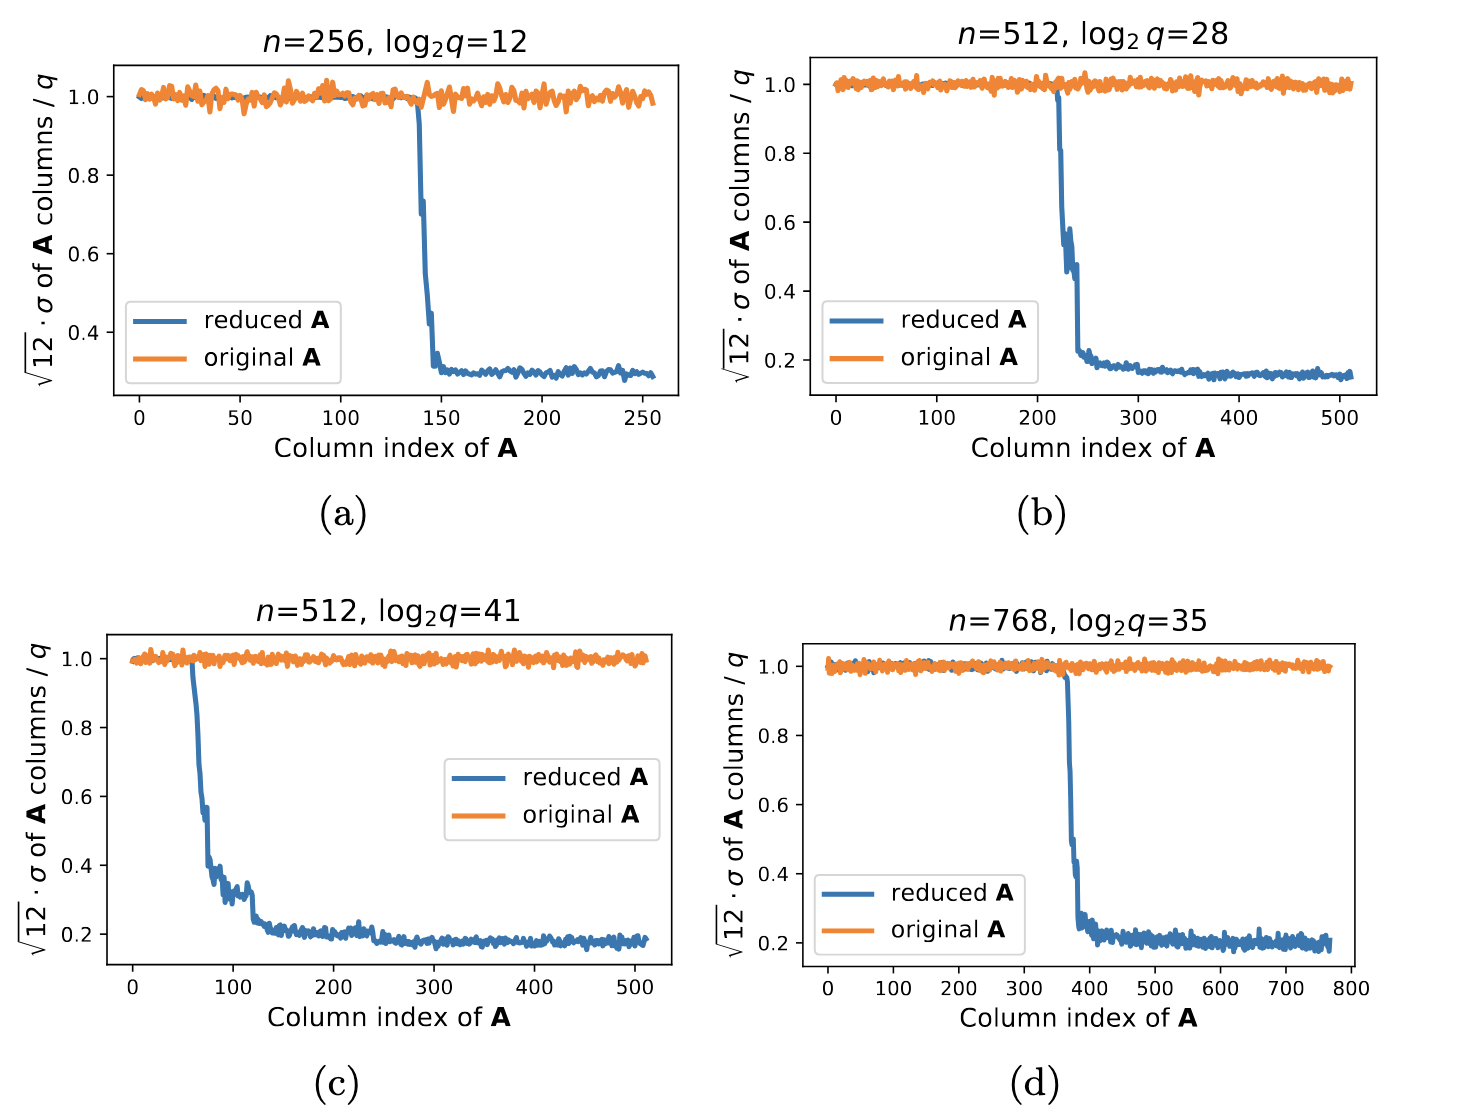
\includegraphics[width=1\linewidth]{example_variance_plot.png} 
  \caption{\small Example variance separation plot: the original matrix $\mathbf{A}$ (orange) has near-uniform column variance $\approx q/\sqrt{12}$, while the reduced matrix $\mathbf{A}'$ (blue) exhibits a sharp drop at index $n_u$.}
  \label{fig:variance-separation}
\end{figure}

\paragraph{Sub-Sampling \& Interleaving.}
Practically, one often \emph{sub-samples} $m$ out of $4n$ or more LWE samples, then runs multiple partial reductions in parallel.
Algorithms like BKZ and \texttt{flatter} can be interleaved, swapping when progress stalls, and final \texttt{polish} steps refine the basis. 
Early termination exports $\mathbf{A}'$ once $\rho$ no longer improves.

\subsection{Greedy Recovery of ``Cool'' Bits}
\label{subsec:greedy}

Following \cite{cool-and-cruel}, if $n_u$ columns remain high variance (``cruel''), one can brute force that subset. 
Once those bits are correct, the remaining $n_r = n - n_u$ columns typically have lower variance (``cool''), allowing a simpler \emph{bit-flip} approach to finalize the secret. 
We summarize it here as \textbf{Algorithm~1}.

\begin{algorithm}[ht]
\caption{\small Greedy Recovery of Cool Bits (from \cite{cool-and-cruel})}
\label{alg:greedy-cool}
\begin{algorithmic}[1]
\Require $\mathbf{s}^*$ partially known (correct cruel bits); the rest initially $=0$.
\For{$i \in \{n - n_r, \ldots, n-1\}$}
  \State $s^*[i] \gets 0$
  \State $\sigma_0 \gets \sigma(\mathbf{A}\cdot \mathbf{s}^* - \mathbf{b}\mod q)$
  \State $s^*[i] \gets 1$
  \State $\sigma_1 \gets \sigma(\mathbf{A}\cdot \mathbf{s}^* - \mathbf{b}\mod q)$
  \If{$\sigma_0 \le \sigma_1$}
    \State $s^*[i] \gets 0$
  \Else
    \State $s^*[i] \gets 1$
  \EndIf
\EndFor
\end{algorithmic}
\end{algorithm}

\noindent
\textbf{Interpretation.}
We individually check whether flipping a particular bit from $0$ to $1$ lowers the residual’s variance; if so, we keep that flip.
This linear-time method works well when each column has \emph{significantly reduced} variance, ensuring a strong statistical signal per bit.

\begin{figure}[ht]
  \centering
  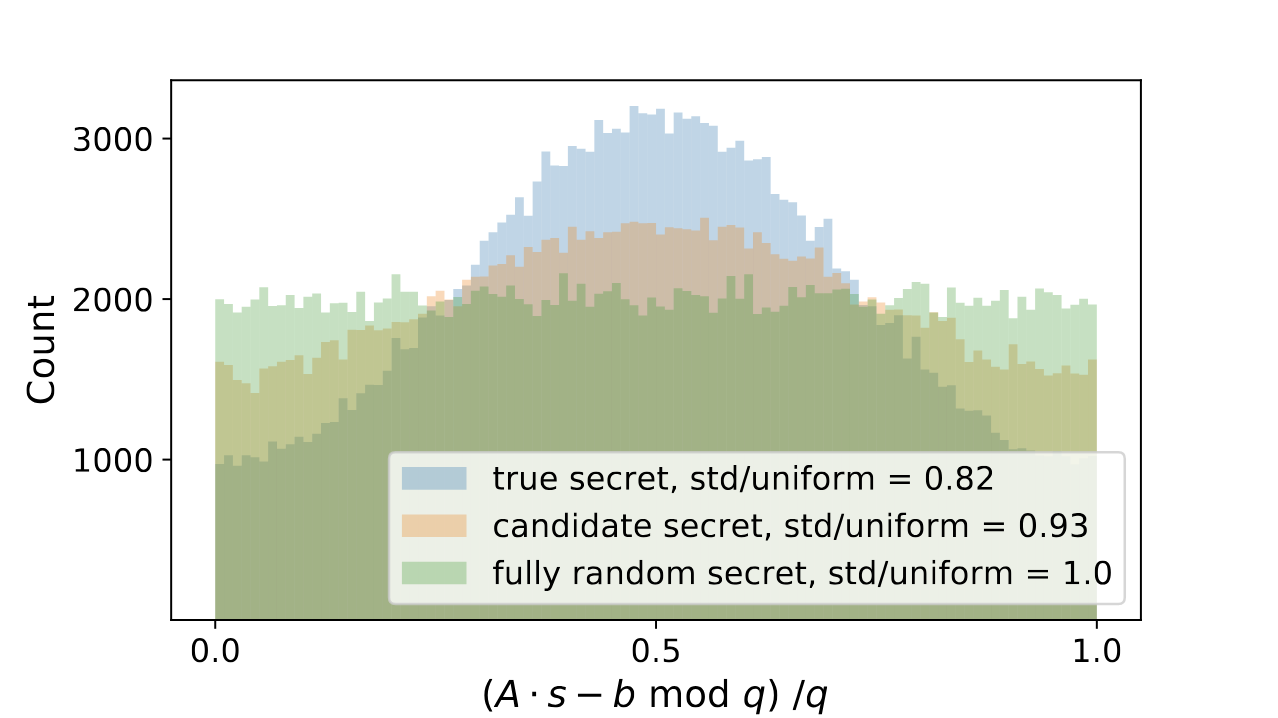
\includegraphics[width=1\linewidth]{residual_histogram.png}
  \caption{\small Residual histograms mod $q$.  
    \textbf{Blue:} True secret guess (narrow distribution),  
    \textbf{Orange:} Partially correct guess (e.g., cruel bits only),  
    \textbf{Green:} Random guess (near-uniform).}
  \label{fig:residual-histograms}
\end{figure}

\paragraph{Limitations.}
When a subset of columns has only \emph{moderately} reduced variance (``sloping''), flipping bits individually can fail if noise remains too large. 
Hence, our proposal in Section~\ref{sec:proposed-ccc} extends beyond a pure \emph{cruel/cool} partition, introducing a ``chill'' region for partial or probabilistic enumeration.

\section{Variance Diagram and Motivation for a Three-Zone Partition}
\label{sec:3zone-motivation}

\subsection{Empirical Observation}
After applying partial lattice reduction to the LWE matrix $\mathbf{A}$, the column-by-column standard deviation often exhibits a near-vertical ``cliff'' in many parameter sets. However, we observe that in some settings, the transition between high variance and low variance can form a \emph{sloping} region rather than a strict step. This phenomenon is shown in Figure~\ref{fig:variance-annotated}, where we have annotated different variance regimes.

\begin{figure}[ht]
    \centering
    \begin{subfigure}{0.49\textwidth}
        \centering
        % Insert your actual figure path:
        \begin{tikzpicture}
            \node[anchor=south west, inner sep=0] (image) at (0,0)
              {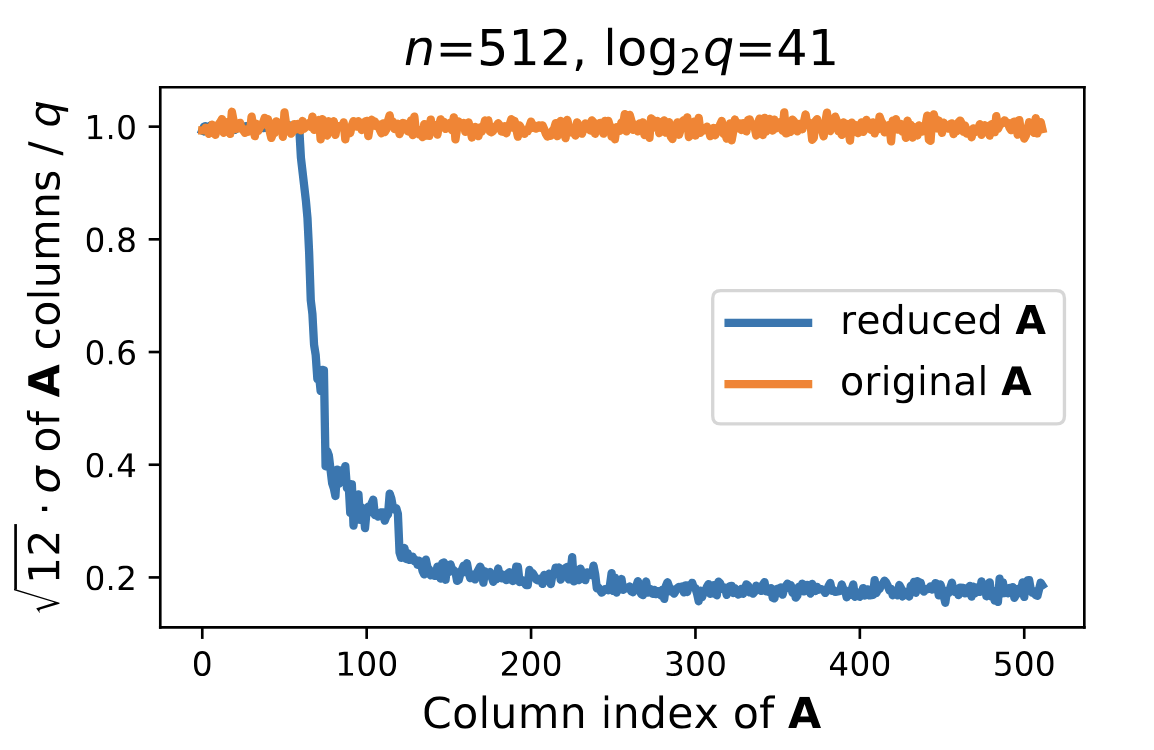
\includegraphics[width=\textwidth]{512-41.png}};
            \begin{scope}[x={(image.south east)}, y={(image.north west)}]
                % Cruel region (green frame)
                \draw[thick, green, fill=green!20, opacity=0.3] (0.18, 0.19) rectangle (0.28, 0.8);
                % Chill region (yellow frame)
                \draw[thick, yellow, fill=yellow!20, opacity=0.3] (0.285, 0.19) rectangle (0.345, 0.8);
                % Cool region (blue frame)
                \draw[thick, blue, fill=blue!20, opacity=0.3] (0.35, 0.19) rectangle (0.91, 0.8);
            \end{scope}
        \end{tikzpicture}
        \caption{\small $n=512, \log_2 q=41$.}
        \label{fig:region1}
    \end{subfigure}
    \hfill
    \begin{subfigure}{0.49\textwidth}
        \centering
        % Insert your actual figure path:
        \begin{tikzpicture}
            \node[anchor=south west, inner sep=0] (image) at (0,0)
              {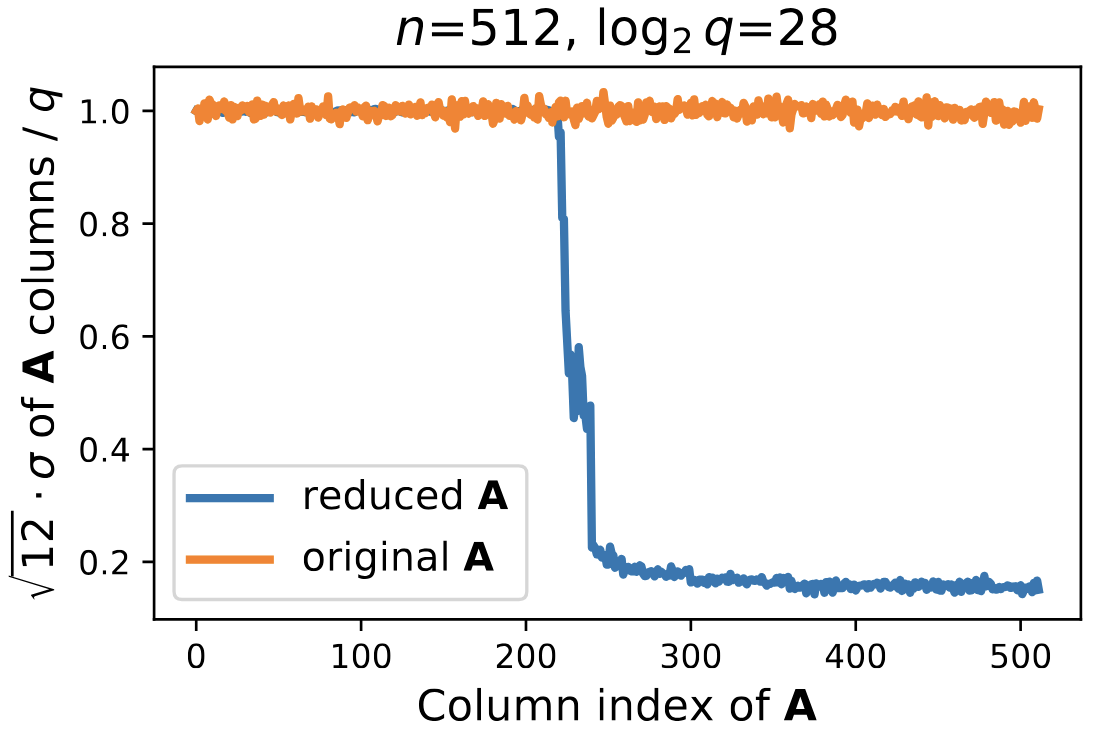
\includegraphics[width=\textwidth]{512-28.png}};
            \begin{scope}[x={(image.south east)}, y={(image.north west)}]
                % Cruel region (green frame)
                \draw[thick, green, fill=green!20, opacity=0.3] (0.18, 0.19) rectangle (0.505, 0.8);
                % Chill region (yellow frame)
                \draw[thick, yellow, fill=yellow!20, opacity=0.3] (0.510, 0.19) rectangle (0.525, 0.8);
                % Cool region (blue frame)
                \draw[thick, blue, fill=blue!20, opacity=0.3] (0.530, 0.19) rectangle (0.935, 0.8);
            \end{scope}
        \end{tikzpicture}
        \caption{\small $n=512, \log_2 q=28$.}
        \label{fig:region2}
    \end{subfigure}
    \caption{\small Empirical plots of column standard deviation (scaled by $\sqrt{12}/q$) before and after reduction, annotated with \textbf{Cruel} (green), \textbf{Chill} (yellow), and \textbf{Cool} (blue) regions. 
    In some instances (left subfigure), the transition from high variance to low variance is relatively narrow, while in others (right subfigure), it forms a longer slope.}
    \label{fig:variance-annotated}
\end{figure}

% Possibly mention that these subfigures correspond to 
% partial-lattice results for dimension n=512, 
% different log2(q), etc.

\paragraph{Why a Slope Can Appear.}
Depending on how \texttt{flatter}, BKZ, or other reduction algorithms interleave, the final column norms might not transition abruptly from $\approx q/\sqrt{12}$ to a fully reduced state. Instead, a fraction of columns may exhibit intermediate ``semi-reduced'' variance, producing what we refer to as a \emph{sloping region}.


\subsection{Why a Three-Zone Partition?}
\label{subsec:3zone}

Historically, ``Cool \& Cruel'' style attacks assumed columns are either:
\begin{itemize}
    \item \emph{Cruel:} High variance $\approx q/\sqrt{12}$, needing brute force or meet-in-the-middle;
    \item \emph{Cool:} Low variance, quickly recovered via bit-flip or minimal overhead.
\end{itemize}
However, a purely two-zone approach \emph{misses} the subtle \emph{middle} region where variance is neither clearly high nor fully reduced. We propose a three-zone decomposition:
\[
  \mathcal{I}_{\mathrm{cruel}},\;
  \mathcal{I}_{\mathrm{chill}},\;
  \mathcal{I}_{\mathrm{cool}}
  \;\subseteq\;\{1,\ldots,n\}, 
  \;\;
\]
\[
  \mathcal{I}_{\mathrm{cruel}}\cup\mathcal{I}_{\mathrm{chill}}\cup\mathcal{I}_{\mathrm{cool}}=\{1,\ldots,n\}.
\]

\begin{itemize}
  \item \textbf{Cruel region (green)}: 
  High-variance columns, roughly uniform $\mathbf{A}_{*,j} \sim q/\sqrt{12}$. 
  We rely on brute force or a hybrid partial guess.
  \item \textbf{Chill region (yellow)}: 
  Transitional/slope columns with \emph{moderate} variance. 
  We treat these with a more refined \emph{probabilistic or ML-based} method, as the noise is not too large to be intractable, yet not so small to do a trivial bit flip.
  \item \textbf{Cool region (blue)}: 
  Columns with significantly reduced variance, for which the standard \emph{greedy flip} approach suffices.
\end{itemize}

\paragraph{Motivation and Potential Approaches.}
\begin{itemize}
    \item \emph{Reduced Overhead:} If the sloping region is assigned a specialized partial-enumeration or machine-learning approach, we avoid fully brute forcing that subset.
    \item \emph{Structured Data:} These transitional columns still hold more structure than the purely uniform cruel bits, giving an ML or statistical classifier a better chance at distinguishing $s_j=0$ vs.\ $s_j=1$.
    \item \emph{Adaptive Windowing:} In practice, we might expand or shrink the chill region if experiments show certain columns can be recovered easily or remain too large in variance.
\end{itemize}

Overall, this \textbf{three-zone} method aims to **bridge** the gap between purely high-variance columns and trivially reduced columns, capturing the “in-between” slope in a dedicated zone for more nuanced cryptanalysis. We formalize the details of each zone’s attack strategy in the next section.

\section{Proposed Method: \texorpdfstring{Cool, Chill, and Cruel}{Cool, Chill, and Cruel}}
\label{sec:proposed-ccc}

\subsection{Threshold-Based Zoning}
\label{subsec:threshold-zoning}

After partially reducing the LWE matrix $\mathbf{A}'$ (Section~\ref{subsec:partial-reduction}), each column $j$ has an associated standard deviation $\sigma_j$. We define two thresholds $T_c$ and $T_h$ with 
\[
  T_c > T_h > 0,
\]
for instance $T_c \approx 0.8 \,\sigma_u$ and $T_h \approx 0.3\, \sigma_u$, where $\sigma_u \approx \frac{q}{\sqrt{12}}$ is the original uniform standard deviation. Then, each column $j$ is classified into one of three regions:
\[
  \mathrm{Region}(j) \;=\;
  \begin{cases}
    \text{Cruel}, & \text{if } \sigma_j \;\ge\; T_c,\\
    \text{Chill}, & \text{if } T_h \;\le\; \sigma_j < T_c,\\
    \text{Cool}, & \text{if } \sigma_j \;<\; T_h.
  \end{cases}
\]
This yields three disjoint subsets $\mathcal{I}_{\mathrm{cruel}}, \mathcal{I}_{\mathrm{chill}}, \mathcal{I}_{\mathrm{cool}} \subseteq \{1,\ldots,n\}$. Figure~\ref{fig:ccc-matrix} illustrates a conceptual $n\times n$ matrix with columns colored green (Cruel), yellow (Chill), and blue (Cool).

\begin{figure}[ht]
  \centering
  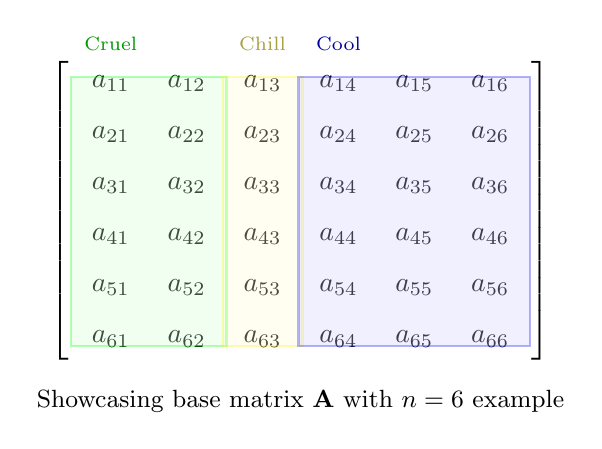
\begin{tikzpicture}[>=stealth, node distance=1.2cm]
  
  %--- Matrix A with coefficients a_ij
  \matrix[matrix of math nodes,
          row sep=0.6em,
          column sep=0.7em,
          left delimiter={[},
          right delimiter={]},
          nodes={minimum size=1em, anchor=center}
          ] (A) {
    a_{11} & a_{12} & a_{13} & a_{14} & a_{15} & a_{16} \\
    a_{21} & a_{22} & a_{23} & a_{24} & a_{25} & a_{26} \\
    a_{31} & a_{32} & a_{33} & a_{34} & a_{35} & a_{36} \\
    a_{41} & a_{42} & a_{43} & a_{44} & a_{45} & a_{46} \\
    a_{51} & a_{52} & a_{53} & a_{54} & a_{55} & a_{56} \\
    a_{61} & a_{62} & a_{63} & a_{64} & a_{65} & a_{66} \\
  };
  
  %--- Highlighting columns for Cruel, Chill, and Cool
  \draw[thick, green, opacity=0.3, fill=green!20]
    ([xshift=-4pt,yshift=-4pt]A-1-1.north west) 
    rectangle ([xshift=4pt,yshift=4pt]A-6-2.south east);
  \node[above=2pt,green!60!black] at (A-1-1.north) {\scriptsize Cruel};
  
  \draw[thick, yellow, opacity=0.3, fill=yellow!20]
    ([xshift=-4pt,yshift=-4pt]A-1-3.north west)
    rectangle ([xshift=4pt,yshift=4pt]A-6-3.south east);
  \node[above=2pt,yellow!60!black] at (A-1-3.north) {\scriptsize Chill};
  
  \draw[thick, blue, opacity=0.3, fill=blue!20]
    ([xshift=-4pt,yshift=-4pt]A-1-4.north west)
    rectangle ([xshift=4pt,yshift=4pt]A-6-6.south east);
  \node[above=2pt,blue!60!black] at (A-1-4.north) {\scriptsize Cool};
  %--- Caption
  \node[below=5pt of A] {\small Showcasing base matrix $\mathbf{A}$ with $n=6$ example};
  
  \end{tikzpicture}
  \caption{Base LWE matrix split into \textbf{Cruel} (green), \textbf{Chill} (yellow), and \textbf{Cool} (blue) column regions. Multiplying by secret $\mathbf{s}$ and adding error $\mathbf{e}$ produces $\mathbf{b}$.}
  \label{fig:ccc-matrix}
\end{figure}


\paragraph{Rationale.}
\begin{itemize}
  \item \textbf{Cruel} ($\sigma_j \approx q/\sqrt{12}$): High variance columns requiring exhaustive or hybrid enumeration.
  \item \textbf{Cool} ($\sigma_j \ll q/\sqrt{12}$): Heavily reduced variance, solvable with a simple bit-flip approach (Algorithm~\ref{alg:greedy-cool}).
  \item \textbf{Chill}: The intermediate zone, where partial enumeration or probabilistic ranking can be significantly cheaper than brute force, yet a naive bit-flip might fail if noise is still moderate.
\end{itemize}


\subsection{Attack Phases}
\label{subsec:attack-phases}

Having classified columns, we propose three sequential phases:

\paragraph{Phase 1: Brute Force (Cruel).}
Columns in $\mathcal{I}_{\mathrm{cruel}}$ remain at near-uniform variance $\approx \frac{q}{\sqrt{12}}$ and must be guessed via:
\[
  \mathrm{BruteForceCruel}(\mathbf{A}_{*, \mathcal{I}_{\mathrm{cruel}}}, \mathbf{b}), 
\]
or a meet-in-the-middle if memory permits. Let $\mathbf{s}_{\mathrm{cruel}}$ be the recovered bits, and $\mathrm{cruel\_ones} = \mathrm{HW}(\mathbf{s}_{\mathrm{cruel}})$ the number of 1-bits found.

\paragraph{Phase 2: Probabilistic Enumeration (Chill).}
The \emph{Chill} region $\mathcal{I}_{\mathrm{chill}}$ has moderate variance. We define a function 
\[
  p_j = \mathrm{EstimateProb}\bigl(j,\mathbf{A},\mathbf{s}_{\mathrm{cruel}}\bigr), \quad
  j \in \mathcal{I}_{\mathrm{chill}},
\]
that ranks columns by the likelihood of $s_j=1$. We then pick $k = h - \mathrm{cruel\_ones}$ bits to set as 1 among $\mathcal{I}_{\mathrm{chill}}$ (or a fraction thereof). If the final check fails, we may refine the guess by local flips or partial enumerations in the Chill region.

\paragraph{Phase 3: Greedy (Cool).}
Finally, for columns in $\mathcal{I}_{\mathrm{cool}}$, the standard \textbf{Greedy Recovery} (Algorithm~\ref{alg:greedy-cool}) is applied. Each bit is flipped if it reduces the standard deviation of the residual $(\mathbf{A}\cdot \mathbf{s}^* - \mathbf{b})\bmod q$. 

\subsection{Pseudocode: Multi-Zone Recovery}
\label{subsec:multi-zone-pseudocode}

Algorithm~\ref{alg:ccc-attack} summarizes the combined approach. We denote a function \textproc{RefineChill} to handle iterative flips in the Chill region if the final solution fails a residual test.

\begin{algorithm}[ht]
\caption{\small Multi-Zone Attack: Cool, Chill, and Cruel}
\label{alg:ccc-attack}
\begin{algorithmic}[1]
\Require Reduced matrix $\mathbf{A}$, vector $\mathbf{b}$, modulus $q$, Hamming weight $h$
\State $(\mathcal{I}_{\mathrm{cruel}},\;\mathcal{I}_{\mathrm{chill}},\;\mathcal{I}_{\mathrm{cool}}) \;\gets\; \text{ClassifyColumns}(\mathbf{A}, T_c, T_h)$
\State $\mathbf{s}_{\mathrm{cruel}} \;\gets\; \mathrm{BruteForceCruel}\bigl(\mathbf{A}_{*,\mathcal{I}_{\mathrm{cruel}}}, \mathbf{b}\bigr)$
\State $\mathrm{cruel\_ones} \gets \mathrm{HW}\bigl(\mathbf{s}_{\mathrm{cruel}}\bigr)$
\State $p_j \;\gets\; \mathrm{EstimateProb}\bigl(j,\mathbf{A},\mathbf{s}_{\mathrm{cruel}}\bigr)\; \text{for}\; j\in \mathcal{I}_{\mathrm{chill}}$
\State $k \;=\; h \;-\; \mathrm{cruel\_ones}$
\State $\mathbf{s}_{\mathrm{chill}} \;\gets\; \mathrm{RankAndAssign}(p_j,\;k)$
\State $\mathbf{s}_{\mathrm{cool}} \;\gets\; \mathrm{GreedyFlip}\bigl(\mathbf{A},\mathbf{b},\mathbf{s}_{\mathrm{cruel}},\mathbf{s}_{\mathrm{chill}}\bigr)$
\State $\mathrm{RefineChill}\bigl(\mathbf{A},\mathbf{b},\mathbf{s}_{\mathrm{cruel}},\mathbf{s}_{\mathrm{chill}},\mathbf{s}_{\mathrm{cool}}\bigr)$
\State \textbf{return} $(\mathbf{s}_{\mathrm{cruel}},\;\mathbf{s}_{\mathrm{chill}},\;\mathbf{s}_{\mathrm{cool}})$
\end{algorithmic}
\end{algorithm}

\paragraph{Implementation Notes.}
\begin{itemize}
\item \textproc{EstimateProb} may rely on column variance or partial distribution checks, potentially combined with small ML models.
\item \textproc{RankAndAssign} sorts columns by $p_j$ descending and picks the top $k$ as 1. A local flip or partial BFS can refine borderline columns.
\item \textproc{GreedyFlip} is the same bit-flip approach described in Section~\ref{subsec:greedy}. 
\end{itemize}

Hence, each region in $\{\mathrm{Cruel, Chill, Cool}\}$ is tackled with a method suited to its variance regime, aiming to minimize overall cost while preserving a high success probability.

\section{Mathematical and Logical Details}
\label{sec:math-logic}

\subsection{Probability and Combinatorial Logic}
\label{subsec:prob-comb}

Once partial-lattice reduction has classified columns into \emph{Cruel, Chill,} or \emph{Cool}, let 
$n_{\mathrm{cruel}}, n_{\mathrm{chill}}, n_{\mathrm{cool}}$ be their respective counts. After enumerating all \emph{cruel} bits, we denote:
\[
  \mathrm{cruel\_1} \;=\; \mathrm{HW}\bigl(\mathbf{s}_{\mathrm{cruel}}\bigr),
\]
the number of ones found in the cruel region. Suppose the total Hamming weight of the secret is $h$. Then 
\[
  k \;=\; h \;-\; \mathrm{cruel\_1}
\]
bits remain to be distributed among Chill and Cool columns.

\paragraph{Probability-Based Ranking (Chill).}  
To determine which $\mathcal{I}_{\mathrm{chill}}$ columns are 1 vs.\ 0, we assign each column $j \in \mathcal{I}_{\mathrm{chill}}$ a probability 
\[
  p_j \;=\; \Pr\bigl[s_j = 1\bigr].
\]
One might define $p_j$ via:
\begin{itemize}
  \item \emph{Heuristic}, e.g.\ $p_j \propto 1 / \sigma_j$,
  \item \emph{Small ML Model}, e.g.\ a logistic regression or shallow neural net trained on partial residual distributions,
  \item \emph{Direct Statistical} test from local distribution checks.
\end{itemize}
Then we can pick $k_{\mathrm{chill}} \le k$ columns to be 1 (the top-$p_j$), with the remainder placed in the cool set.

\paragraph{Local Search if Wrong Guess.}  
If the final check fails or residual distribution indicates errors, a small BFS or iterative local flip approach can refine which columns in $\mathcal{I}_{\mathrm{chill}}$ are set to 1. This \emph{partial search} tries to correct borderline columns without enumerating the full $\binom{n_{\mathrm{chill}}}{k_{\mathrm{chill}}}$ space.

\subsection{Complexity Insights}
\label{subsec:complexity}

We approximate the overall cost by combining:
\begin{itemize}
  \item \emph{Brute Force} on $\mathcal{I}_{\mathrm{cruel}}$,
  \item \emph{Chill Enumerations} (or local BFS),
  \item \emph{Cool Overhead}, typically linear in $n_{\mathrm{cool}}$.
\end{itemize}

\vspace{1em}
\noindent\textbf{Notional Complexity Formula.}
\begin{align*}
\mathbf{C}(n, k)
  &\approx\; 
  2^{n_{\mathrm{cruel}}} 
  \;+\;
  \binom{\textstyle n_{\mathrm{chill}}}{\textstyle k_{\mathrm{chill}}}
  \times\; \mathrm{ML\_overhead}(1) 
  \times\;
\end{align*}

\vspace{-5mm}

\noindent
\begin{align*}
    &\times\;
    \Bigl[
    1 \;+\; \mathrm{liability\_coef}
        \;\times\;
        \bigl(
          n \;-\; n_{\mathrm{cruel}} \;-\; n_{\mathrm{chill}}
        \bigr)
  \Bigr] =
\end{align*}

\vspace{-3mm} % Reduce space between equations

\noindent
\begin{align*}
&= 2^{\,n_{\mathrm{cruel}}} 
     \;+\; 
     \lunderbrace{\binom{\textstyle n_{\mathrm{chill}}}{\textstyle k_{\mathrm{chill}}} 
       \times \mathrm{ML\_overhead}(1) 
       \times
       \bigl[ 1 + }_{\text{chill enumerations}}
\end{align*}
       
\vspace{-5mm} % Reduce space between equations

\noindent
\begin{flalign*}
    &\runderbrace{ + \mathrm{liability\_coef}\times(\dots) \bigr]}_{\text{chill enumerations}} 
     \;+\;
     \underbrace{(\dots)}_{\text{cool overhead}}
\end{flalign*}



\paragraph{Term-by-Term Explanation.}
\begin{enumerate}
  \item \(\mathbf{2^{n_{\mathrm{cruel}}}}\): 
  Exhaustive or meet-in-the-middle enumeration for the truly high-variance columns.

  \item \(\binom{n_{\mathrm{chill}}}{k_{\mathrm{chill}}}\):
  Worst-case enumerations for deciding which bits are 1 among the chill columns (if we enumerated fully). In practice, we rely on ranking or partial BFS to reduce real cost.

  \item \(\mathrm{ML\_overhead}(1)\):
  Additional time per candidate guess, e.g.\ a small neural net pass or advanced statistical test. 
  If no ML is used, this overhead may be a simpler partial check.

  \item \(\mathrm{liability\_coef}\times(\dots)\):
  Models repeated local flips or expansions if the initial chill guess fails. The factor \((n - n_{\mathrm{cruel}} - n_{\mathrm{chill}})\) can interpret how each fix might need re-running the “cool” step or re-sampling for distribution tests.

  \item \(\text{cool overhead}\):
  Typically $O(n_{\mathrm{cool}})$ from the final bit-flip approach, or a minimal additive cost for verifying correct bits in a heavily reduced domain.
\end{enumerate}

\paragraph{Comparison to Original Cool-and-Cruel.}
In \cite{cool-and-cruel}, columns are labeled either ``hard'' ($n_u$ bits to brute force) or ``easy'' (linear-time flips). The complexity is roughly
\[
  2^{n_{u}} \;+\; O(n - n_u).
\]
Where \[
n_u \approx n_{\mathrm{cruel}}.
\]

That approach can fail or become costly if many columns exhibit \emph{medium} variance. By contrast, our three-zone method invests partial enumerations or an ML-based routine in that “chill” portion, potentially lowering $n_{\mathrm{cruel}}$ (fewer bits in the brute force set) at the expense of the extra $\binom{n_{\mathrm{chill}}}{k_{\mathrm{chill}}}$ (chill) overhead.

\subsection{Balancing Reduction and Secret Recovery}
\label{subsec:balance}

One can tune the partial reduction parameter $\omega$ to achieve fewer cruel columns ($n_{\mathrm{cruel}}$) at the risk of amplifying noise $\sigma_e$ in the chill or cool region. Overly strong reduction may hamper the final bit-flip step or the probability ranking approach, while insufficient reduction leaves $n_{\mathrm{cruel}}$ large. An \emph{adaptive} or \emph{incremental} strategy might re-run partial reduction if the brute force dimension is still too big or if the chill region is too uncertain. We leave a deeper analysis of this trade-off to future work, noting that the sweet spot depends heavily on dimension $n$, modulus $q$, and the desired security level.

\section{Discussion, Future Work, and Conclusion}
\label{sec:discussion-future-conclusion}

\subsection{Discussion}
Our three-zone (\emph{Cruel}, \emph{Chill}, \emph{Cool}) approach addresses columns whose variance after partial lattice reduction does not form a perfect “cliff.” Instead, we isolate a \emph{Chill} region to treat medium-variance columns more effectively than a pure two-zone partition. By combining:
\begin{itemize}
    \item brute force (or meet-in-the-middle) on the \emph{Cruel} subset,
    \item a probabilistic or ML-driven ranking for the \emph{Chill} subset, 
    \item and a greedy bit-flip for the \emph{Cool} subset,
\end{itemize}
we hope to reduce both worst-case and average-case runtime when a substantial sloping region emerges. The notional complexity analysis in Section~\ref{sec:math-logic} showed how partial enumerations in the Chill region can replace an overly large brute force set, albeit with some overhead for classification or local refinement.

\paragraph{Balancing Lattice Reduction.}
One key observation (Section3, p.8 in \cite{cool-and-cruel}) is that stronger partial reduction lowers $n_{\mathrm{cruel}}$ but increases the noise $\sigma_e$, which can hamper correct classification of bits in Chill and Cool. Hence, an adaptive or incremental approach—where we tune the penalty parameter $\omega$ and the block sizes in BKZ/\texttt{flatter}—may offer an optimal middle ground. Future experiments are needed to measure the trade-off between enumerating more \emph{cruel} bits vs.\ dealing with bigger error in Chill/Cool columns.

\subsection{Future Work}
Below we outline the main directions for refining and evaluating our method:

\paragraph{1.\ Ternary/Gaussian Secrets.}
While we have focused on sparse \emph{binary} LWE, many HE systems experiment with ternary or narrow Gaussian secret distributions. Extending our Chill-based classification to these distributions could require adjusted probability estimates or separate ML training. The magnitude of partial reduction might further complicate these multi-valued secrets.

\paragraph{2.\ Combining with SALSA or Transformers.}
Recent works (e.g., SALSA, PICANTE, VERDE) use neural networks or transformer models for partial or full key recovery. Our Chill region could incorporate similar models as the “local classification” step, potentially improving accuracy if moderate-variance columns are effectively recognized. However, careful overhead management is crucial, since a large ML model could increase the $(\mathrm{ML\_overhead})$ term in our complexity formula.

\paragraph{3.\ Real-World Library Impact and Mitigations.}
Beyond purely theoretical settings, open-source HE libraries (e.g., HElib, SEAL) often rely on small or sparse secrets. System designers might mitigate three-zone attacks by randomizing the distribution of secrets, enforcing a minimum Hamming weight, or rotating sub-lattices to obfuscate partially reduced columns. Investigating each library’s susceptibility to a Chill-based enumeration is an important step in bridging the gap between cryptanalysis and real deployments.

\paragraph{4.\ Parameter Tuning and Local Search.}
In the Chill region, local flips or BFS expansions can drastically reduce enumerations, yet we lack a formal rule for how many flips or restarts are cost-effective. Defining “liability coefficients,” cost functions, or iteration bounds remains an open question. Tuning these parameters is critical for achieving practical speedups while ensuring a high probability of correct guesses.

\paragraph{5.\ Incrementally Expanding the Chill Window.}
Another approach is to \emph{iteratively} decide which columns belong to Chill vs.\ Cool. For instance, one might start with a small Chill region, attempt partial classification, then gradually expand it if columns in the borderline zone are incorrectly guessed as Cool. Experimental data will reveal how such window adjustments affect final runtime and success rates.

\begingroup
Note: implementation of the new approach will take the existing original Cool and Cruel implementation as the base. Src can be viewed at: \cite{lwe-benchmarking}.
\endgroup

\subsection{Conclusion}
In this work, we introduced a \emph{Cool, Chill, and Cruel} partition to address the limitations of a purely two-zone approach for partial-lattice-based LWE key recovery. By classifying columns into high-variance (\emph{Cruel}), moderate-variance (\emph{Chill}), and low-variance (\emph{Cool}) regimes, we tailor each subset’s recovery method—ranging from brute force to statistical or ML-based partial enumeration, and finally a greedy bit-flip. Our complexity analysis suggests that while the Chill region adds overhead in the worst case, it may substantially reduce the overall search space compared to letting those columns remain in a large brute force set.

We anticipate further gains by fine-tuning the partial lattice reduction depth ($\omega$), exploring advanced classification for Chill columns, and adapting local search heuristics. Empirical tests with parameter sets up to $n=1024$ (and potentially higher) will help confirm whether this approach is practical against real-world homomorphic encryption libraries and ring-based LWE implementations. By unifying classical cryptanalytic strategies with modern ML insights, we hope to push forward the state of cryptanalysis on small or sparse LWE secrets.

  \bibliographystyle{plain}
  \bibliography{references}

\end{document}